\documentclass[10pt,pdf,hyperref={unicode}]{beamer}

\mode<presentation>
{
\usetheme{boxes}
\beamertemplatenavigationsymbolsempty

\setbeamertemplate{footline}[page number]
\setbeamersize{text margin left=1em, text margin right=0.5em}
}

\usepackage[utf8]{inputenc}
\usepackage[english, russian]{babel}
\usepackage[normalem]{ulem}
\usepackage{bm}
\usepackage{multirow}
\usepackage{ragged2e}
\usepackage{indentfirst}
\usepackage{multicol}
\usepackage{subfig}
\usepackage{amsmath,amssymb}
\usepackage{dsfont}
\usepackage{enumerate}
\usepackage{mathtools}
\usepackage{comment}
\usepackage{tabularx, tabulary, multicol}
\usepackage[all]{xy}

\newcommand{\bz}{\mathbf{z}}
\newcommand{\bx}{\mathbf{x}}
\newcommand{\by}{\mathbf{y}}
\newcommand{\bv}{\mathbf{v}}
\newcommand{\bw}{\mathbf{w}}
\newcommand{\ba}{\mathbf{a}}
\newcommand{\bb}{\mathbf{b}}
\newcommand{\bff}{\mathbf{f}}
\newcommand{\bh}{\mathbf{h}}
\newcommand{\bl}{\mathbf{l}}
\newcommand{\bp}{\mathbf{p}}
\newcommand{\bq}{\mathbf{q}}
\newcommand{\bs}{\mathbf{s}}
\newcommand{\bt}{\mathbf{t}}
\newcommand{\bu}{\mathbf{u}}
\newcommand{\bT}{\mathbf{T}}
\newcommand{\bX}{\mathbf{X}}
\newcommand{\bZ}{\mathbf{Z}}
\newcommand{\bS}{\mathbf{S}}
\newcommand{\bH}{\mathbf{H}}
\newcommand{\bW}{\mathbf{W}}
\newcommand{\bY}{\mathbf{Y}}
\newcommand{\bU}{\mathbf{U}}
\newcommand{\bQ}{\mathbf{Q}}
\newcommand{\bP}{\mathbf{P}}
\newcommand{\bA}{\mathbf{A}}
\newcommand{\bB}{\mathbf{B}}
\newcommand{\bC}{\mathbf{C}}
\newcommand{\bE}{\mathbf{E}}
\newcommand{\bF}{\mathbf{F}}
\newcommand{\bsigma}{\boldsymbol{\sigma}}
\newcommand{\bomega}{\boldsymbol{\omega}}
\newcommand{\btheta}{\boldsymbol{\theta}}
\newcommand{\bgamma}{\boldsymbol{\gamma}}
\newcommand{\bdelta}{\boldsymbol{\delta}}
\newcommand{\bPsi}{\boldsymbol{\Psi}}
\newcommand{\bpsi}{\boldsymbol{\psi}}
\newcommand{\bxi}{\boldsymbol{\xi}}
\newcommand{\bmu}{\boldsymbol{\mu}}
\newcommand{\bchi}{\boldsymbol{\chi}}
\newcommand{\bzeta}{\boldsymbol{\zeta}}
\newcommand{\blambda}{\boldsymbol{\lambda}}
\newcommand{\beps}{\boldsymbol{\varepsilon}}
\newcommand{\bZeta}{\boldsymbol{Z}}
% mathcal
\newcommand{\cX}{\mathcal{X}}
\newcommand{\cY}{\mathcal{Y}}
\newcommand{\cW}{\mathcal{W}}

\newcommand{\dH}{\mathds{H}}
\newcommand{\dR}{\mathds{R}}
% transpose
\newcommand{\T}{^{\mathsf{T}}}

% command to strike out text
\newcommand{\stkout}[1]{\ifmmode\text{\sout{\ensuremath{#1}}}\else\sout{#1}\fi}

% limited alertblock
\newenvironment<>{varblock}[2][.9\textwidth]{%
	\setlength{\textwidth}{#1}
	\begin{actionenv}#3%
		\def\insertblocktitle{#2}%
		\par%
		\usebeamertemplate{block begin}}
	{\par%
		\usebeamertemplate{block end}%
	\end{actionenv}}

\renewcommand{\epsilon}{\ensuremath{\varepsilon}}
\renewcommand{\phi}{\ensuremath{\varphi}}
\renewcommand{\kappa}{\ensuremath{\varkappa}}
\renewcommand{\le}{\ensuremath{\leqslant}}
\renewcommand{\leq}{\ensuremath{\leqslant}}
\renewcommand{\ge}{\ensuremath{\geqslant}}
\renewcommand{\geq}{\ensuremath{\geqslant}}
\renewcommand{\emptyset}{\varnothing}

\usepackage{tikz}
\usetikzlibrary{positioning,arrows}

\tikzstyle{name} = [parameters]
\definecolor{name}{rgb}{0.5,0.5,0.5}

\usepackage{caption}
\captionsetup{skip=0pt,belowskip=0pt}

\newtheorem{rustheorem}{Теорема}
\newtheorem{russtatement}{Утверждение}
\newtheorem{rusdefinition}{Определение}

% colors
\definecolor{darkgreen}{rgb}{0.0, 0.2, 0.13}
\definecolor{darkcyan}{rgb}{0.0, 0.55, 0.55}

\AtBeginEnvironment{figure}{\setcounter{subfigure}{0}}

\captionsetup[subfloat]{labelformat=empty}
\addto\captionsrussian{\renewcommand{\figurename}{}}
\graphicspath{{../figures/}}

%----------------------------------------------------------------------------------------------------------

\title[Заголовок]{Генеративный причинно-следственный подход к анализу данных ИМК}
\author{Владимиров Э.А.}

\institute[]{Московский физико-технический институт}
\date{\footnotesize
	\par\smallskip\emph{Научный руководитель:} д.~ф.-м.~н. В.\,В.~Стрижов
	\par\bigskip\small 2023}

%---------------------------------------------------------------------------------------------------------
\begin{document}

\begin{frame}
\titlepage
\end{frame}

%----------------------------------------------------------------------------------------------------------
\begin{frame}{Причинно-следственный анализ}
	\begin{alertblock}{Проблема}
		\begin{itemize}
			\item Традиционные методы (корреляция, линейная регрессия) неадекватны для сложных нелинейных связей
			\item Данные имеют высокую размерность, что усложняет поиск причинно-следственных связей
			\item Зависимости между переменными могут изменяться во времени
		\end{itemize}
	\end{alertblock}
	
	\begin{alertblock}{Решение}
		Построить устойчивую и интерпретируемую форму вероятностного анализа причинного влияния $\bX \rightarrow \bY$
	\end{alertblock}
\end{frame}

%---------------------------------------------------------------------------------------------------------
\begin{frame}{Различные подходы к поиску связей}
	\begin{multicols}{2}
		\begin{figure}
			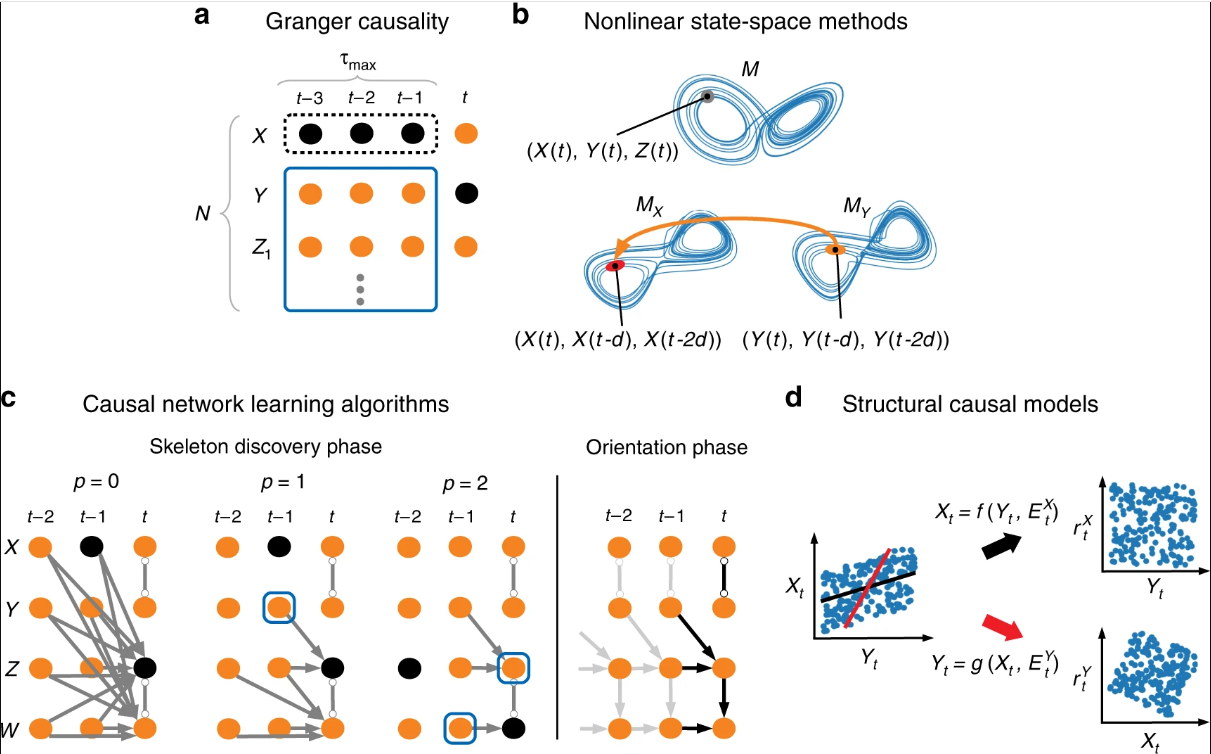
\includegraphics[width=\linewidth]{ci-approaches}
			\caption{Существующие подходы}
		\end{figure}
	
		\begin{figure}
			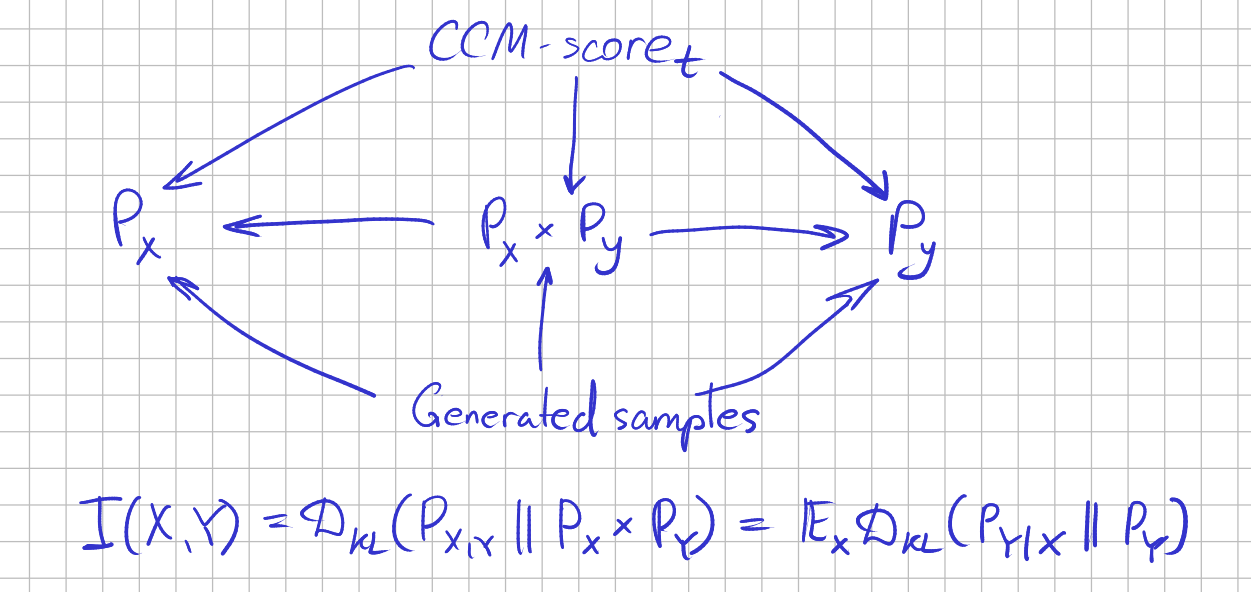
\includegraphics[width=\linewidth]{ccm-prob.png}
			\caption{Предлагаемый подход}
		\end{figure}
	\end{multicols}
\end{frame}

%--------------------------------------------------------------------------------------------------------

\begin{frame}{Постановка задачи}
	Пусть \( \mathbf{X}(t) = \{X_1(t), X_2(t), \ldots, X_{n_x}(t)\} \) и \( \mathbf{Y}(t) = \{Y_1(t), Y_2(t), \ldots, Y_{n_y}(t)\} \) — два набора многомерных временных рядов, наблюдаемых в моменты времени \( t = 1, \ldots, T \).
	
	Необходимо определить направленные причинные связи:
	\begin{enumerate}
		\item \( X_i(t-\tau) \to Y_j(t) \) для \( i = 1, \ldots, n_x \), \( j = 1, \ldots, n_y \), и лагов \( \tau \geq 0 \),
		\item \( Y_j(t-\tau) \to X_i(t) \) для \( i = 1, \ldots, n_x \), \( j = 1, \ldots, n_y \), и лагов \( \tau \geq 0 \).
	\end{enumerate}
	
	Предполагаем, что многомерные временные ряды \( \mathbf{X}(t) \) и \( \mathbf{Y}(t) \) генерируются следующим образом:
	\[
	X_i(t) = f_i(\text{Pa}_{X_i}(t), \varepsilon_{X_i}(t)),
	\]
	\[
	Y_j(t) = g_j(\text{Pa}_{Y_j}(t), \varepsilon_{Y_j}(t)),
	\]
	где:
	\begin{itemize}
		\item \( \text{Pa}_{X_i}(t) \subseteq \{Y_1(t-\tau), \ldots, Y_{n_y}(t-\tau)\} \) — множество родителей переменной \( X_i(t) \) из \( \mathbf{Y} \),
		\item \( \text{Pa}_{Y_j}(t) \subseteq \{X_1(t-\tau), \ldots, X_{n_x}(t-\tau)\} \) — множество родителей переменной \( Y_j(t) \) из \( \mathbf{X} \),
		\item \( f_i \) и \( g_j \) — детерминированные функции, описывающие зависимость,
		\item \( \varepsilon_{X_i}(t) \) и \( \varepsilon_{Y_j}(t) \) — шумовые компоненты.
	\end{itemize}
\end{frame}

\begin{frame}
	Оптимизационная задача:
	\[
	\min_{G_{XY}, G_{YX}} \mathcal{L}(\mathbf{X}, \mathbf{Y} \mid G_{XY}, G_{YX}) + \lambda_1 \mathcal{R}(G_{XY}, G_{YX}) + \lambda_2 \mathcal{T}(G_{XY}, G_{YX}),
	\]
	где:
	\begin{itemize}
		\item \( G_{XY} \) — граф зависимостей \( X_i \to Y_j \),
		\item \( G_{YX} \) — граф зависимостей \( Y_j \to X_i \),
		\item \( \mathcal{L}(\mathbf{X}, \mathbf{Y} \mid G_{XY}, G_{YX}) \) — правдоподобие наблюдаемых данных с учетом графов \( G_{XY} \) и \( G_{YX} \),
		\item \( \mathcal{R}(G_{XY}, G_{YX}) \) — регуляризатор, штрафующий за сложность графов,
		\item \( \mathcal{T}(G_{XY}, G_{YX}) \) — штраф за избыточную изменчивость графов во времени.
	\end{itemize}
\end{frame}

%---------------------------------------------------------------------------------------------------------
\begin{frame}{Independent Component Analysis}
	Предположим, что $\mathbf{X}(t)$ образуется из нескольких скрытых источников $\mathbf{S}(t)\in \mathbb{R}^{d_S}$:
	\[
		\mathbf{X}(t) \;=\; A\,\mathbf{S}(t), 
		\quad
		A \in \mathbb{R}^{d_X \times d_S}.
	\]
	
	Каждая компонента $S_k(t)$ предполагается статистически независимой от других:
		\[
		p(\mathbf{S}) = \prod_{k=1}^{d_S} p\bigl(S_k\bigr).
		\]
	
	\textbf{Задача оптимизации:}
		Найти обратную матрицу $\widehat{A}^{-1}$, дающую
		\[
		\widehat{\mathbf{S}}(t) 
		\;=\; 
		\widehat{A}^{-1}\,\mathbf{X}(t),
		\]
		чтобы минимизировать взаимную информацию между компонентами $\widehat{S}_k(t)$.
		\[
		\mathrm{MI}\bigl(\widehat{\mathbf{S}}(t)\bigr) 
		\;\approx\; 
		\sum_{k=1}^{d_S} H\bigl(S_k\bigr) - H\Bigl(\sum_k S_k\Bigr),
		\]

\end{frame}
%----------------------------------------------------------------------------------------------------------
\begin{frame}{Convergent Cross Mapping}
	\textbf{Теневое вложение (delay embedding):}
	\[
	M_{X,t}
	= 
	\bigl(
	X_t,\,
	X_{t-\tau},\,
	\dots,\,
	X_{t-(E-1)\tau}
	\bigr)
	\;\in\;\mathbb{R}^E,
	\]
	где $E$ --- размерность вложения, $\tau$ --- временной лаг. Аналогично задаётся 
	$
	M_{Y,t} = \bigl(Y_t,\,Y_{t-\tau},\,\dots\bigr).
	$
	
	\vspace{1em}
	\textbf{Реконструкция:}
	\[
	\widehat{Y}_t
	=
	\sum_{i=1}^{k}
	w_i\,
	Y_{n_i},
	\]
	здесь $n_i$ --- индексы ближайших соседей точки $M_{X,t}$ в пространстве $M_X$, а $w_i$ --- веса, зависящие от расстояния до $M_{X,t}$.
	
	\vspace{1em}
	\textbf{Критерий причинности:}
	\[
	\rho_{X\to Y}
	=
	\mathrm{corr}\!\Bigl(\{\widehat{Y}_t\},\{Y_t\}\Bigr).
	\]
	Если при увеличении размера ``библиотеки'' (количества доступных точек) значение $\rho_{X\to Y}$ \emph{возрастает}, считается, что $\mathbf{X}(t)$ действительно влияет на $\mathbf{Y}(t)$.
\end{frame}

%----------------------------------------------------------------------------------------------------------
\begin{frame}{Probabilistic CCM}
	\textbf{Идея:} Вместо единственного прогноза $\widehat{Y}_t$ рассматривается \emph{полное условное распределение} 
	\[
	p_L\bigl(Y_t \mid M_{X,t}\bigr),
	\]
	оценённое по выборке размера $L$. Ближайшие соседи в пространстве $M_X$ позволяют построить \emph{вероятностную аппроксимацию} (например, ядерным методом):
	
	\[
	p_L\bigl(y \mid M_{X,t}\bigr)
	\;=\;
	\frac{1}{Z_t}
	\sum_{i \in N_L(t)}
	K\Bigl(y - Y_{n_i}\Bigr),
	\]
	где $K(\cdot)$ --- ядро (например, гауссово), $N_L(t)$ --- множество соседей точки $M_{X,t}$, а $Z_t$ --- нормировочная константа.
	
	\vspace{1em}
	\textbf{Оценка причинности как MI:}
	\[
	I_L\bigl(X \to Y\bigr)
	\;=\;
	\mathbb{E}_{\hat{M_{X, t}}}
	D_{\mathrm{KL}}\!\Bigl(
	p_L\bigl(Y_t \mid \hat{M_{X,t}}\bigr)
	\;\big\|\;
	p\bigl(Y_t\bigr)
	\Bigr),
	\]
	
	\vspace{1em}
	\textbf{Сходящееся свойство:}  
	При $L \to \infty$ (при достаточно плотном покрытии пространства)  
	\[
	p_L\bigl(Y_t \mid M_{X,t}\bigr)
	\;\to\;
	p\bigl(Y_t \mid M_{X,t}\bigr),
	\]

\end{frame}

%----------------------------------------------------------------------------------------------------------
\begin{frame}{Предлагаемый метод}
	\begin{enumerate}
		\item \textbf{Независимый анализ компонент (ICA).}\\
		Для исходных ЭЭГ-данных $\mathbf{X}_{\mathrm{raw}}(t)\in\mathbb{R}^{d_X}$ получаем независимые компоненты:
		\[
		\widehat{\mathbf{S}}(t) 
		= 
		\widehat{A}^{-1}\,\mathbf{X}_{\mathrm{raw}}(t).
		\]
		
		\vspace{0.5em}
		\item \textbf{Построение эмбеддингов.}\\
		Для каждого времени $t$ формируем вектор:
		\[
		M_{X,t} = 
		\bigl(\widehat{\mathbf{S}}(t),\,\widehat{\mathbf{S}}(t-\tau),\dots,\widehat{\mathbf{S}}(t-(E-1)\tau)\bigr),
		\]
		
		\vspace{0.5em}
		\item \textbf{Оценка причинно-следственных связей.}\\
		В полученном пространстве $(M_{X,t},\,M_{Y,t})$ определяем меру влияния $\mathbf{X}\to\mathbf{Y}$, вычисляя:
		\[
		\gamma(t)
		=
		\mathrm{Prob-CCM}\bigl(M_{X,t},\,M_{Y,t}\bigr).
		\]
		Результат --- временной ряд $\{\gamma(t)\}$, отражающий динамику влияния $X\to Y$.
		
	\end{enumerate}
\end{frame}

%----------------------------------------------------------------------------------------------------------
\begin{frame}{Риманова постановка задачи}
	Причинно-следственная связь ~--- вероятность push-forward-а или диффеоморфизма.
	
	Основная проблема ~--- построение многообразий
	
	Возможные варианты:
	\begin{itemize}
		\item PINN
		\item Riemannian space of covariance matrices
	\end{itemize}
\end{frame}

%----------------------------------------------------------------------------------------------------------
\begin{frame}{Вычислительный эксперимент на данных ЭЭГ - ИИМ}	
	\begin{multicols}{2}
	
		\begin{varblock}[6cm]{Данные}
			У 25 участников были записаны показания ЭЭГ, ИИМ, МРТ во время игры в настольный теннис. С каждым участником было сыграно 4 сессии, длительность каждой из них составляет 7-10 минут.
		\end{varblock}
	
		\begin{figure}
			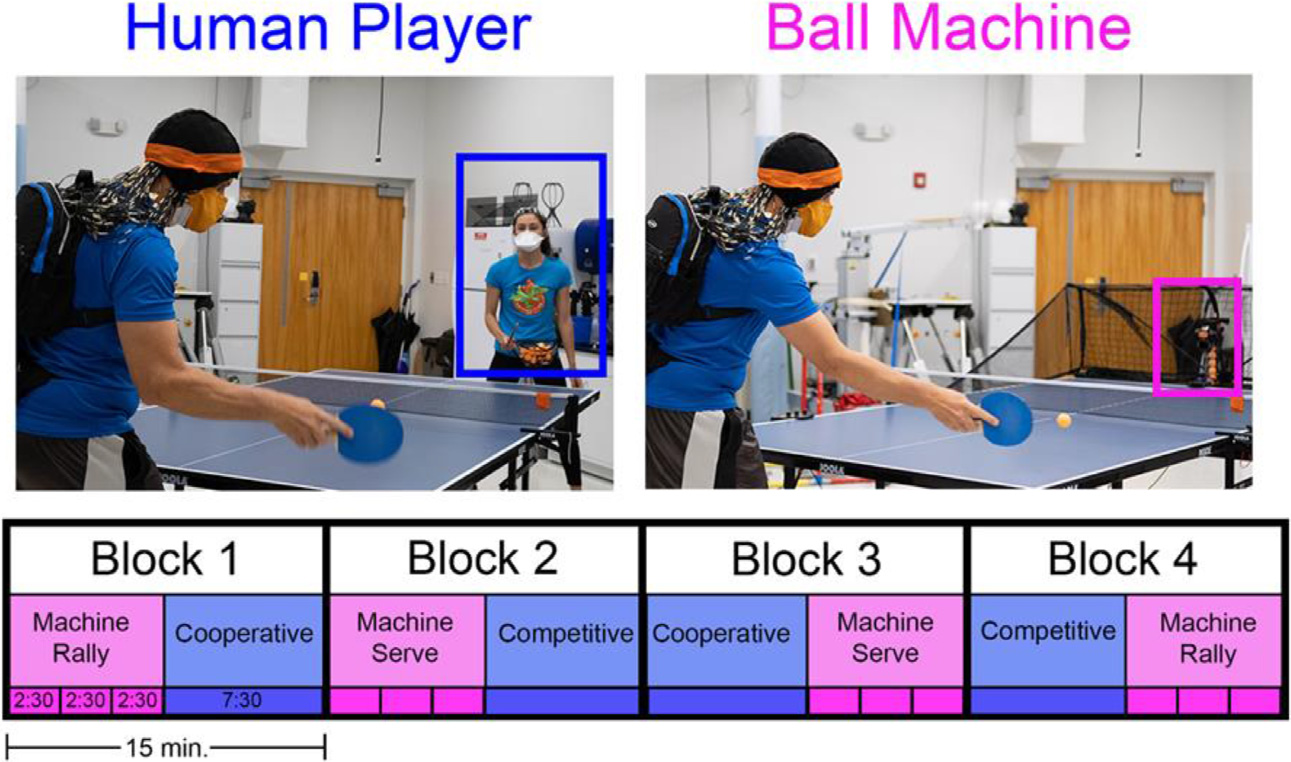
\includegraphics[width=\linewidth]{tennis-viz.png}
		\end{figure}
	
	\end{multicols}
\end{frame}


\end{document} 
